%%%%%%%%%%%%%%%%%%%%%%%%%%%%%%%%%%%%%%%%%%%%%%%%%%%%%%%%%%%%%%%%%%%%%
%% The same is true for Supporting Information, which should use the
%% suppinfo environment.
%%%%%%%%%%%%%%%%%%%%%%%%%%%%%%%%%%%%%%%%%%%%%%%%%%%%%%%%%%%%%%%%%%%%%
\begin{suppinfo}

This will usually read something like: ``Experimental procedures and
characterization data for all new compounds. The class will
automatically add a sentence pointing to the information on-line:
\section{Dataset}
Here have a summary of all the fragment data

\section{Samples from different SILVR rates}
\begin{figure}
    \centering
    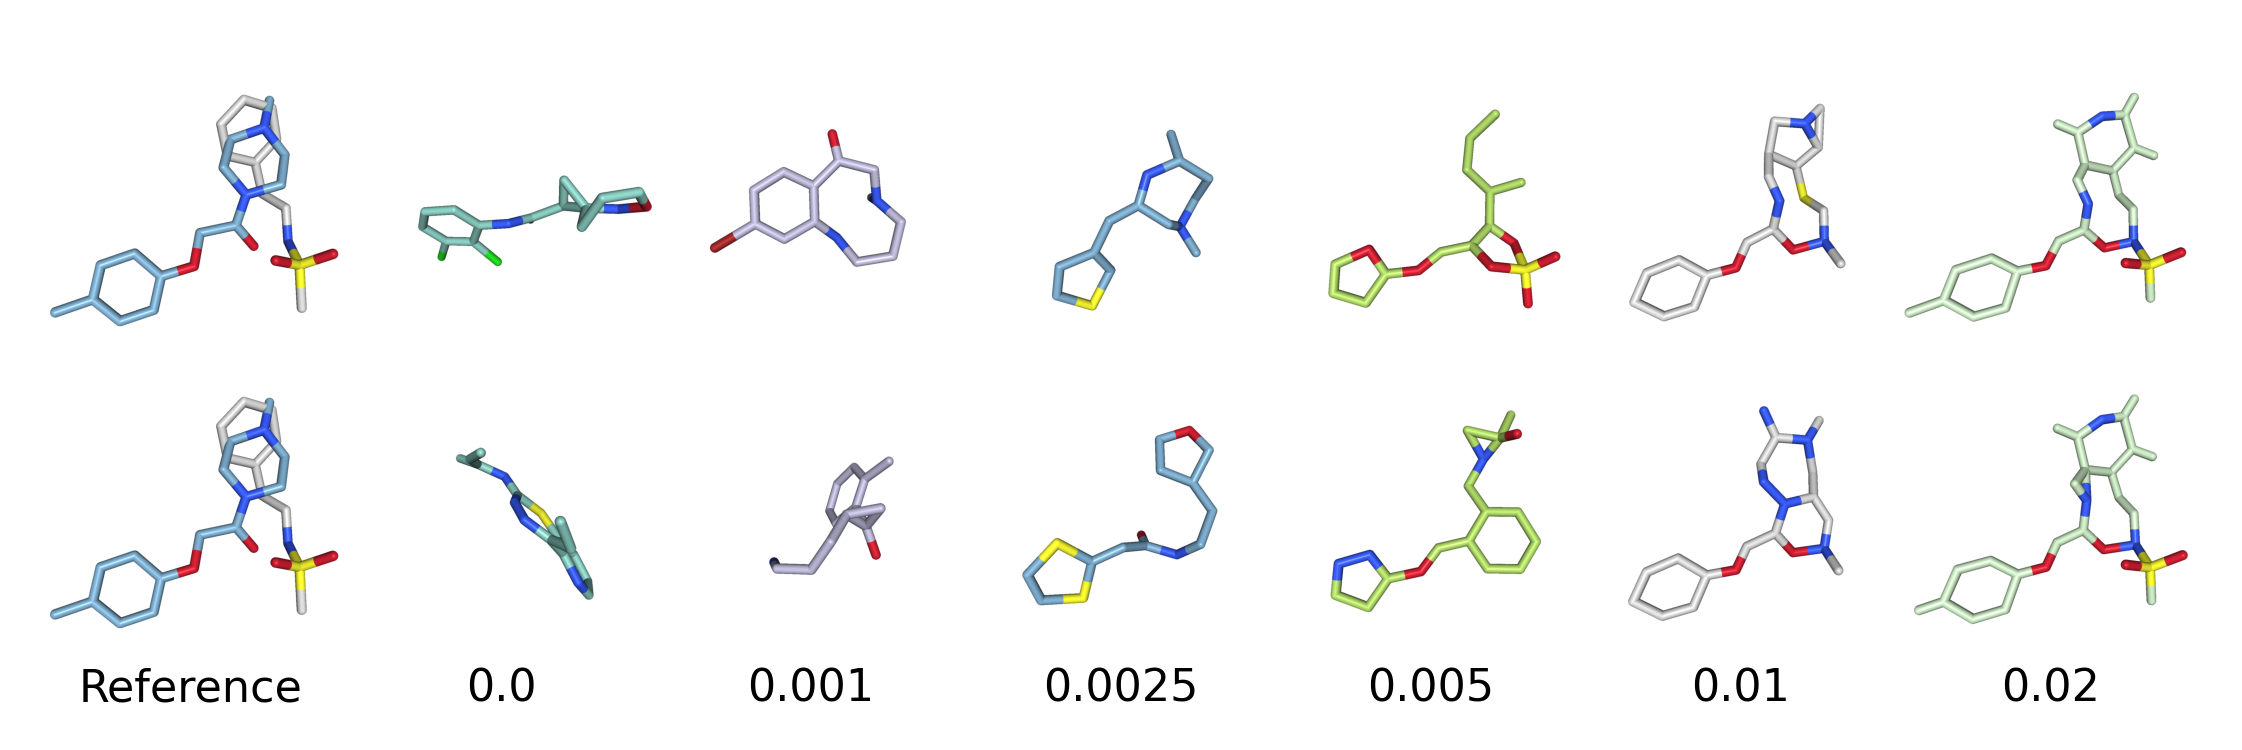
\includegraphics[width=\textwidth]{paper/Figures/FigS2/fig_2_sample_vs_rate.png}
    \caption{Two random samples from the same reference using different SILVR rates. All bonds were inferred from XYZ coordinates with openbabel. All bonds were visualised as single bonds and hydrogen atoms were deleted for clarity. Increasing SILVR rate results in sampled atom coordinates coming closer in space, and element type, to the reference while still resembling a true molecular structure.}
    \label{fig:fig_2}
\end{figure}


\end{suppinfo}